\documentclass{article}%
\usepackage[T2A]{fontenc}%
\usepackage[utf8]{inputenc}%
\usepackage{lmodern}%
\usepackage{textcomp}%
\usepackage{lastpage}%
\usepackage[russian]{babel}%
\usepackage{titling}%
\usepackage{nopageno}%
\usepackage{amsfonts}%
\usepackage{amssymb}%
\usepackage{amsmath}%
\usepackage[left=2cm,right=2cm, top=2cm,bottom=2cm]{geometry}%
\usepackage{circuitikz}%

\begin{document}%

\begin{titlepage}
  \begin{center}
    \large
    Министерство образования Республики Беларусь\\
    \vspace{0.5cm}
    БЕЛОРУССКИЙ ГОСУДАРСТВЕННЫЙ УНИВЕРСИТЕТ
    \vspace{0.5cm}
     
    Факультет прикладной математики и информатики
\bigskip
\vfill
\vfill
\vfill
\vfill
\centerline{\Large \bf Лабораторная работа 2}
    \vspace{0.5cm}
\centerline{"Метод сеток решения краевой задачи для ОДУ"}
\end{center}

\vspace*{\fill}
\vfill
\vfill
\vfill
\hfill
\begin{minipage}{0.25\textwidth}
{   Подготовил:\\ студент 3 курса 3 группы\\ Тев Никита Михайлович\\}
\end{minipage}

\mbox{}
\vfill
\hfill
\begin{minipage}{0.25\textwidth}
  {\large{\bf Преподаватель: } 
{\it\\ Горбачёва Юлия \\ Николаевна}}
\end{minipage}

\vspace*{\fill}
\vfill
\vfill
\vfill
\vfill
\vfill
\vfill
\vfill
\vfill
\vfill
\vspace*{\fill}
\begin{center}
Минск, 2019 г.
\end{center}
\end{titlepage}

\begin{enumerate}%
\item%
\underline{Постановка задачи}

Дана линейная краевая задача. 
Необходимо построить для краевой задачи разностную схему второго порядка аппроксимации на минимальном шаблоне и с помощью метода прогонки при $h = 0.05$ найти её численное решение. 
Оценить погрешность полученного численного решения с помощью правила Рунге. 
Обосновать применимость метода прогонки для решения разностной задачи. Построить график численного решения задачи.

\item%
\underline{Условие задачи:}

$\begin{cases} 
u''(x) + (\frac{1}{3} - x)u'(x) - (x^2-1)u(x)=sinx,\,  0<x<1\\ u'(0) - u(0) = 1 \\ u(1) = 1
\end{cases}$

\item%
\underline{Построение разностной схемы}

Примем следующие обозначения:

$\begin{cases} 
p(x) = (\frac{1}{3} - x) \\ q(x) = (x^2-1) \\ f(x) = sinx
\end{cases}$

Тогда исходная задача примет вид:

$\begin{cases} 
u''(x) + p(x)u'(x) - q(x)u(x)=f(x),\,  0<x<1\\ u'(0) - u(0) = 1 \\ u(1) = 1
\end{cases}$

\vskip 0.2in

Построим разностную схему:

$\begin{cases} 
y_{{\overline x}x}(x) + p(x)y_{\overset{o}{x}}(x) - q(x)y(x)=f(x),\,  0<x<1\\ y_x(0) + ay(0) = b \\ y(1) = 1
\end{cases}$

Чтобы получить метод второго порядка точности, необходимо подобрать соответствующие коэффициенты a и b.

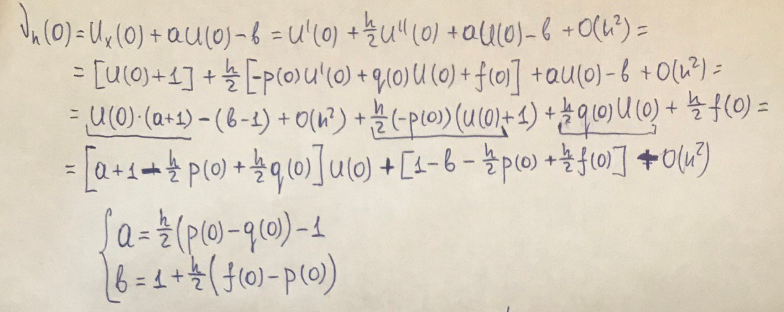
\includegraphics[scale=0.7]{lab2_2_0.png}

$\begin{cases} 
a = \frac{h}{2}(p(0)-q(0)) - 1 \\ b =\frac{h}{2}(f(0)-p(0))+1
\end{cases}$

Перейдем к индесной форме и найдем коэффициенты прогонки.

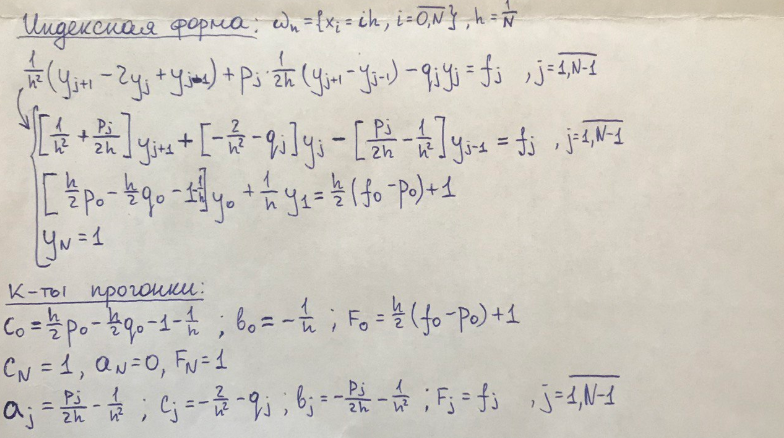
\includegraphics[scale=0.7]{lab2_2_1.png}

Докажем корректность и утсойчивость метода прогонки. Для найденных коэффициентов выполняются неравенства:

$|c_0|\geq|a_0|$

$|c_i|\geq|a_i|, 1<i<N-1$

$|c_N|>|a_N|$

Значит, можно применять метод прогонки.

\item%
\underline{Листинг программы}



\begin{verbatim}
\end{verbatim}

\item%
\underline{Результаты работы}

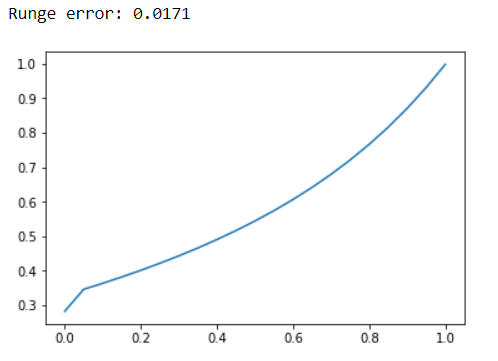
\includegraphics[scale=0.7]{lab2_2_results.png}
\end{enumerate}%
\end{document}